\newcommand{\package}{\emph}

\setcounter{chapter}{1}
\setcounter{section}{0}
\section{Problem 1: Logistic difference equation}
We can find stable points from  
\begin{equation}
f(x, a) = ax(1-x) = x
\label{eq:p01_main}
\end{equation}
as the roots of the quadratic equation:
\begin{equation}
ax^2 - (a - 1)x = x(ax - (a - 1)) = 0
\end{equation}
which are:
\begin{align}
x_1 &= 0 \\
x_2 &= \frac{(a-1)}{a}
\end{align}
The fixed point $x_2$ is non-negative if $a \geq 1$.
One can analyze the local stability of the difference equation \ref{eq:p01_main} by examining the partial derivative of $f$ with respect to $x$ evaluated at each fixed point $x^{\ast}$:
\begin{equation}
f' = - ax - a(x - 1)
\label{eq:p01_diffmain}
\end{equation}

Substituting $x_1$ and $x_2$ into \ref{eq:p01_diffmain} yields:
\begin{align}
f'(x_1) &= a \\
f'(x_2) &= 2 - a
\end{align}

One finds that if $a>1 \rightarrow f'(x_1) > 1 $ with $x_1 = 0$, then $x^{\ast}$ is repelling, while if $1 < a < 3 \rightarrow 1 > f'(x_2) > -1 $ with $x_2 = (a - 1) / a$ is stable (attractor).

\subsection{Point stability at different values of $a$}

When $a = 0.9$ then $x_1 = 0.9, x_2 = 1.1$ \\
When $a = 2.1$ then $x_1 = 2.1, x_2 = -0.1$

For $a$ values in excess of $3.57$, the orbits $x(t, x0) = {x0, x1, x2, ... }$ depend crucially on the initial condition $x0$. Slight variations in $x0$ result in dramatically different orbits, an important characteristic of chaos.

\begin{figure}[h]
 \centering
    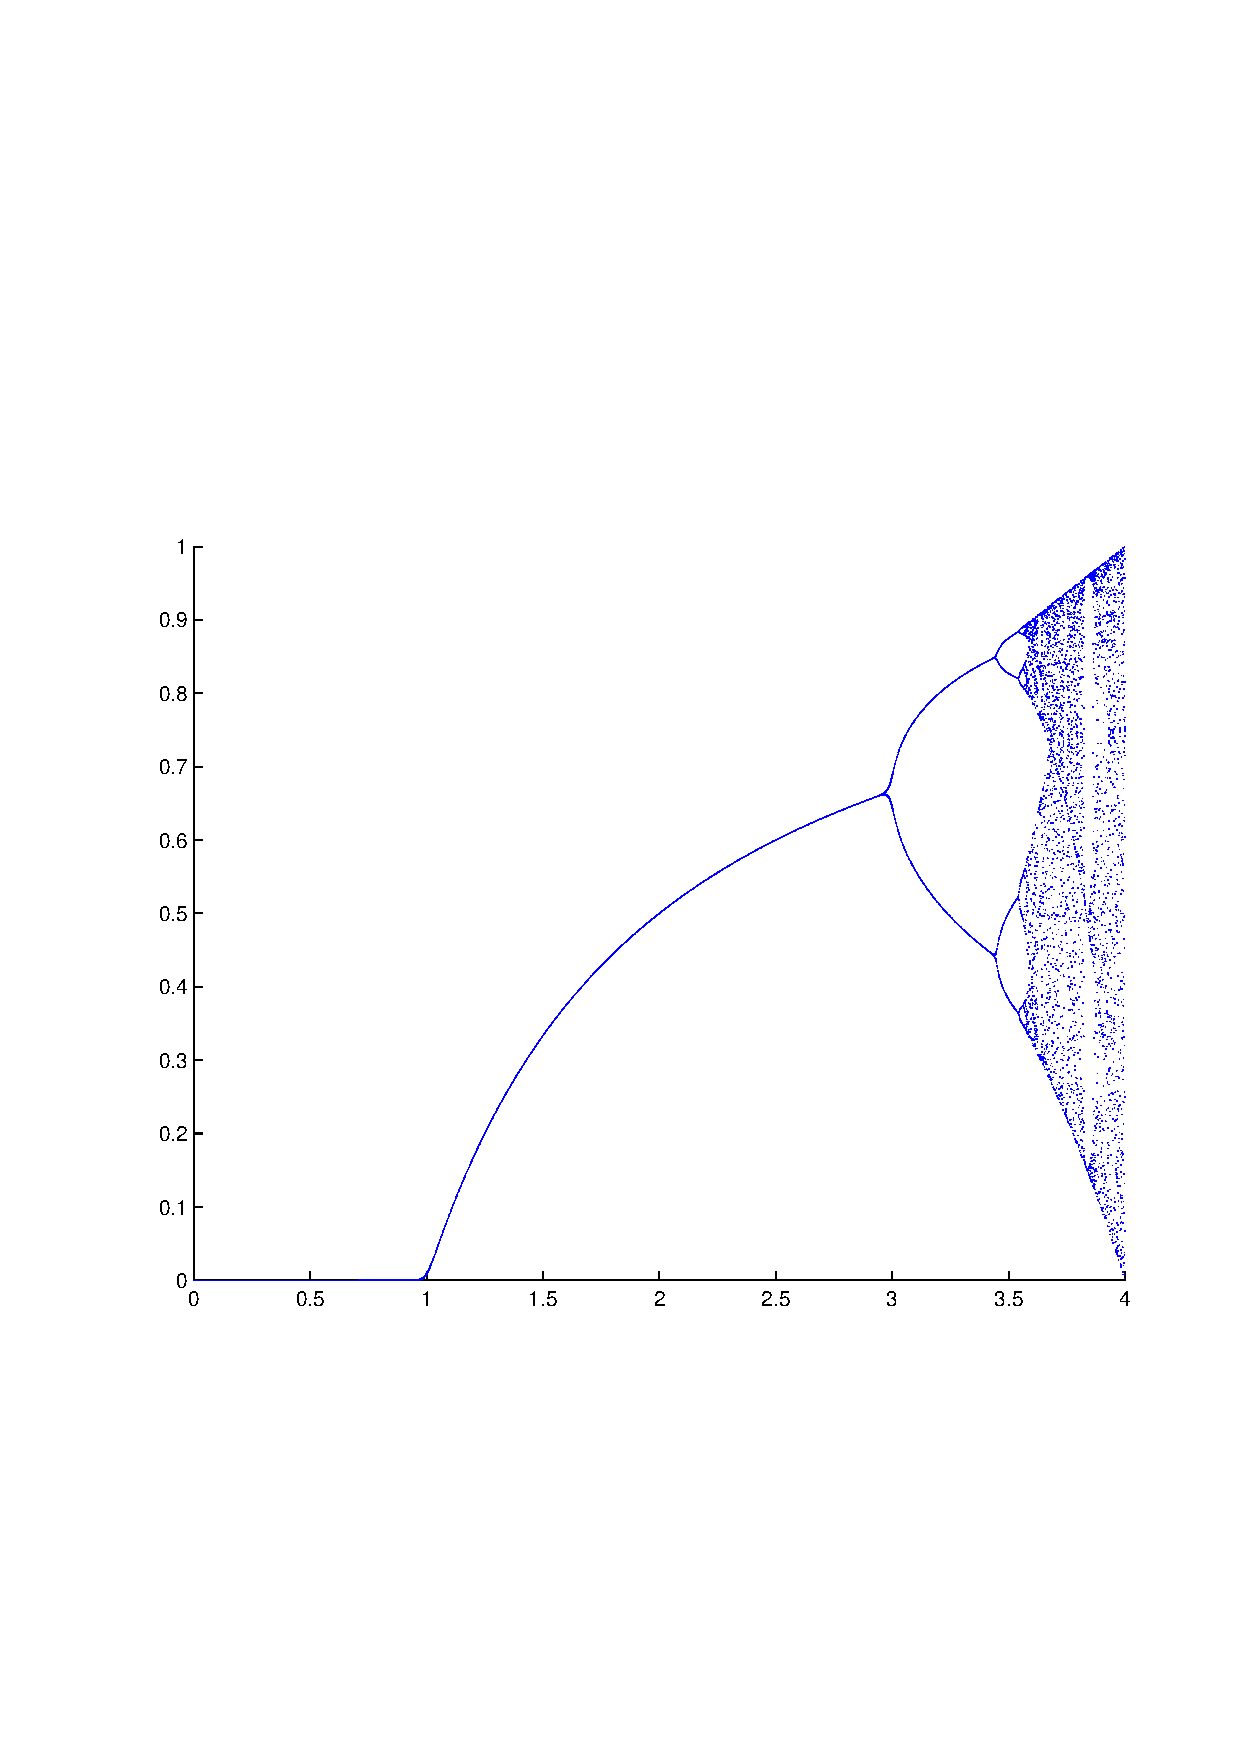
\includegraphics[scale=0.55]{plot_A01_P01.pdf}
    \caption{Logistic Map Bifurcation Diagram}
	\label{fig:plot_logistic_map_bifgraph}
\end{figure}


\setcounter{chapter}{2}
\setcounter{section}{0}
\section{Problem 2: Logistic growth in continuous time}
We have to solve the equation
\begin{equation}
\frac{dx}{dt} = rx (1-\frac{x}{K})  = r(x - \frac{x^2}{K}) = \frac{rx(K-x)}{K}
\label{eq:p02_main}
\end{equation}
using the separation of variables
\begin{equation}
\frac{K}{x(K-x)}dx = rdt
\end{equation}
decomposing the right part with partial fractions
\begin{equation}
\frac{K}{x(K-x)}=\frac{A}{x} + \frac{B}{K-x}
\end{equation}
We find A and B
\begin{align}
A&= \frac{K - Bx}{K-x} \\
B &= \frac{K-A(K-x)}{x}
\end{align}
Supposing $A = 1$, and according to above, $B$ is also equal to $1$, so our partial fraction decomposition is
\begin{equation}
\frac{K}{x(K-x)}=\frac{1}{x} + \frac{1}{K-x}
\end{equation}
Now we have to take the integral from both parts:
\begin{align}
\int{\frac{1}{x}+\frac{1}{K-x}dx} &= \int{rdt}\\
\int{\frac{1}{x}}+\int{\frac{1}{K-x}dx} &= r\int{dt}\\
\ln{x} - \ln{K-x} &= rt + x_0\\
\ln{\frac{x}{K-x}} &= rt + x_0\\
\frac{x}{K-x} &= x_0e^{rt}
\end{align}
Finally the solution 
\begin{equation}
x(t) = x_0Ke^{rt}\frac{1}{K + x_0(e^{rt}-1)}
\end{equation}

\subsection{Determining the stability of equilibria}

To determine the stability of the two equilibria points found solving the equation \ref{eq:p02_main} in $0$
\begin{align}
x_1 &= 0\\
x_2 &= K
\end{align}
one has to derive it for $x$:
\begin{equation}
f' = - r(\frac{x}{K} - 1) - \frac{rx}{K}\\
\label{eq:p02_diffmain}
\end{equation}
Substituting $x_1$ and $x_2$ into \ref{eq:p02_diffmain} yields:
\begin{align}
f'(x_1) &= -1 \\
f'(x_2) &= -r
\end{align}

One finds that if $ f'(x_1) $ with $x_1 = 0$, then $x^{\ast}$ is always stable, while if $ for r < 0 \rightarrow f'(x_2) > 0 $ with $x_2 = -r $ $x^{\ast}$ is repelling.



\setcounter{chapter}{3}
\setcounter{section}{0}
\section{Problem 3: Hardy-Weinberg equilibrium}

\setcounter{chapter}{4}
\setcounter{section}{0}
\section{Problem 4: Sequence alphabets}

\setcounter{chapter}{5}
\setcounter{section}{0}
\section{Problem 5: Random sequences}

\setcounter{chapter}{6}
\setcounter{section}{0}
\section{Problem 6: Quasispecies}